% Blackboard submission reference: 01097342-4ccd-49fe-93f3-f345930abf45

\documentclass{article}
\usepackage[utf8]{inputenc}
\usepackage{multicol}
\usepackage{listings}
\usepackage{amssymb}
\usepackage{enumitem}
\usepackage{graphicx}
\usepackage{amsthm}
\usepackage{hyperref}
% \usepackage[letterpaper, landscape, margin=1in]{geometry}
\usepackage[ruled,vlined]{algorithm2e}

\usepackage{tikz}
\usetikzlibrary{arrows}

\newtheorem{theorem}{Theorem}
\newtheorem{definition}{Definition}

\SetKwFunction{WriteLn}{WriteLn}
\SetKwFunction{display}{display}
\SetKwFunction{chooseElement}{chooseElement}
\SetKwFunction{findCycle}{findCycle}
\SetKwFunction{cc}{cc}
\SetKwFunction{DFS}{DFS}
\SetKwFunction{DFSVisit}{DFSVisit}
\SetKwFunction{checkGraph}{allVerticesAreReachable}
\SetKwFunction{checkVertexStates}{checkVertexStates}
\SetKwProg{Fn}{Function}{}{}
\SetKwProg{Proc}{Procedure}{}{}




%=====================================
%		    Assignment 3
%=====================================

\begin{document}

\title{Weekly Assignment 3}
\date{\today}
\author{Tony Lopar s1013792}
\maketitle

\paragraph{Deadline:} 27th September 2017, 6pm.
\paragraph{Solutions can be found below the exercises}


\section*{Exercise 1.}
Apply DFS to the graph below. Give values of $d[u]$ and $f[u]$ for all vertices $u$. Draw the DFS tree.

% \begin{figure}[h!]
% \centering
% \includegraphics[width=5cm]{images/[Algo]Week3_Exercise1.png}
% \end{figure}
% \vspace*{-0.5cm}

\subsection*{Solutions exercise 1}
For this solution we will assume that the vertices are in an incrementing order in the graph.

\begin{enumerate}
    \item We start by giving vertex 1 the discovery time 1. We scan all it's adjecents: this are 2, 3 and 4
    \item We continue to vertex 2 and give it discovery time 2. We scan all its adjectent and see that it has none. We give this vertex finishing time 3.
    \item We go back to predecessor vertex 1. We continue by giving vertex 3 the discovery time 4 and we scan all his adjecents and find 5 and 6.
    \item We go further to 5 and give it the discovery time 5. We scan it's adjecents and only find the already discovered 3. We give vertex 5 the finishing time 6.
    \item We continue with the next adjecent of vertex 3, namely vertex 6 and give it the discovery time 7. All adjecents are discovered, so we give it finishing time 8.
    \item We go back to 3 and give it finishing time 9.
    \item We go back to 1 and start discovering it's next adjecent, namely vertex 4. We give this adjecent discovery time 10.
    \item The only adjecent is the already discovered 3, so we give 4 the finishing time 11.
    \item We discovered all adjecents of 1 and give it the finishing time 12.
\end{enumerate}

A visual representation of the graph after dfs can be found in the image below. In this image the discover and finishing times are shown for all vertices and the depth-first tree is shown by red edges. The predecessor of each vertex is given by the green lines.
% \begin{figure}[h!]
% \centering
% \includegraphics[width=5cm]{images/[Algo]Week3_Exercise1_Tree.png}
% \end{figure}
\begin{center}
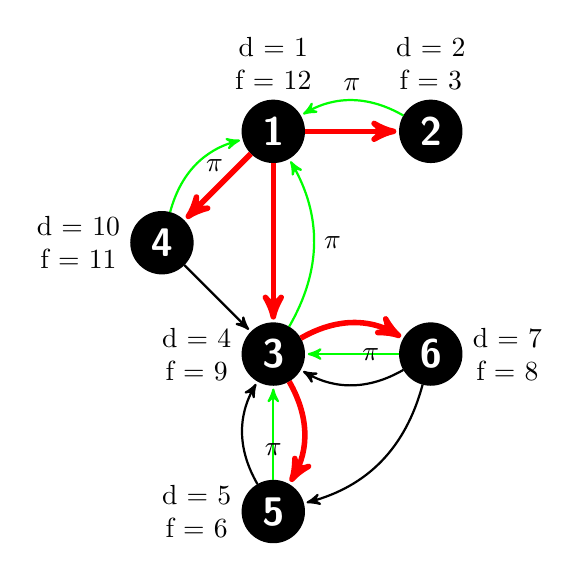
\begin{tikzpicture}[->,>=stealth',shorten >=1pt,auto,node distance=2cm, every loop/.style={},
                    thick, ,main node/.style={circle,draw,font=\sffamily\Large\bfseries}]

  \node[fill = black, text = white, label = {[align=center]above:d = 1\\f = 12}][main node] (1) {1};
  \node[fill = black, text = white, label = {[align=center]above:d = 2\\f = 3}][main node] (2) [ right of=1] {2};
  \node[fill = black, text = white, label = {[align=center]left:d = 10\\f = 11}][main node] (4) [below left of=1] {4};
  \node[fill = black, text = white, label = {[align=center]left:d = 4\\f = 9}][main node] (3) [below right of=4] {3};
  \node[fill = black, text = white, label = {[align=center]left:d = 5\\f = 6}][main node] (5) [ below of=3] {5};
  \node[fill = black, text = white, label = {[align=center]right:d = 7\\f = 8}][main node] (6) [ right of=3] {6};

  \path[every node/.style={font=\sffamily\normalsize, text = black }]
    (1) edge[red, line width=2pt] node [below] {} (2)
        edge[red, line width=2pt] node [left] {} (3)
        edge[red, line width=2pt] node [below] {} (4)
    (2) edge[bend right, green] node [above] {$\pi$} (1)
    (3) edge[bend left, red, line width=2pt] node [left] {} (5)
        edge[bend right, green] node [right] {$\pi$} (1)
        edge[bend left, red, line width=2pt] node [above] {} (6)
    (4) edge[black] node [left] {} (3)
        edge[bend left, green] node [right] {$\pi$} (1)
    (5) edge[bend left, black] node [left] {} (3)
    (5) edge[left, green] node [below] {$\pi$} (3)
    (6) edge[bend left, black] node [left] {} (3)
        edge[left, green] node [right] {$\pi$} (3)
        edge[bend left, black] node [left] {} (5);
\end{tikzpicture}
\end{center}
\vspace*{-0.5cm}


\section*{Exercise 2.}

Most graph algorithms that take an adjacency-matrix representation
as input require time $O(|V|^2)$, but there are some exceptions. Show
how to determine whether a directed graph $G = (V,E)$ contains a \emph{universal sink}, i.e., a vertex with in-degree $n - 1$ and out-degree $0$, in time $O(|V|)$ given an adjacency matrix for $G$.

\subsection*{Solutions exercise 2}
An universal sink is a vertex with no adjacencies from it, but all other vertices point to it. In an adjacency matrix the row with the universal sink will only contain 0 and the column will only contain 1, except on the column with the sink node itself. An adjacency matrix with of a graph with a universal sink could look like this:

\vspace{0.2cm}
\begin{center}
    \begin{tabular}{c|c|c|c|c|c|}
         & $u$ & $v_1$ & $v_2$ & $v_3$ & $v_4$ \\
        \hline
        $u$     & 0 & 0 & 0 & 0 & 0\\
        $v_1$   & 1 & 0 & 0 & 0 & 0 \\
        $v_2$   & 1 & 0 & 0 & 0 & 0 \\
        $v_3$   & 1 & 0 & 0 & 0 & 0 \\
        $v_4$   & 1 & 0 & 0 & 0 & 0 \\
    \end{tabular}
\end{center}
\vspace{0.2cm}
Since in this example there are only edges that point to the universal sink, we can pick two random vertices and pick their value from the matrix. These two vertices should not be equal. For every pair $(u, v)$ for which we search the value in the matrix. If the value is 0, then $v$ can't be the universal sink and otherwise $u$ can't be the universal sink. With this process, after every comparation we can drop one value from the list of possible universal sinks. This means that after $|V| - 1$ comparations, only one possible vertex should remain.
\newpage
\section*{Exercise 3.}

Give an efficient algorithm which takes as input a directed graph $G = (V,E)$, and determines whether or not
there is a vertex $s \in V$ from which all other vertices are reachable.

\subsection*{Solutions exercise 3}
The algorithm will use DFS to decide whether all vertices are reachable. For every vertex we will call a DFS-visit until we found a vertex that reaches all other vertices. After the DFS-visit from a vertex we will check whether all vertices in the graph are finished(no white vertices in the graph). If this is the case, then we found a vertex from which we can reach all other vertices and we will return true. Otherwise, we will make all vertices undiscovered to make sure all vertices that are discovered are reached from one specific vertex. After that we will continue with a DFS-visit on the next vertex. If we haven't found a node after all vertices, then there is no vertex which reaches all other vertices, so we return false.
\begin{algorithm}[ht!]
  \DontPrintSemicolon

    \Proc{\checkGraph{G}}{

        \ForEach{$u \in V$}{
            \DFSVisit{u} \;
            \If{\checkVertexStates{G} }{
                \KwRet{true}
            } \Else{
                \ForEach{$x \in V$}{
                    $color[x] = white$ \;
                }
            }
        }
        \KwRet{false}
    }
    \Proc{\checkVertexStates{G}}{
        \ForEach{$u \in V$}{
            \If{$color[u] = white$}{
                \KwRet{false}
            }
        }
        \KwRet{true}
    }
    \caption{Check whether all vertices are reachable}
\end{algorithm}



\newpage
\section*{Exercise 4.}
A student has to write an algorithm to find a cycle in an directed graph, that is to say, given a graph $G$, find cycle ($x_1$, $\ldots x_{k-1}$, $x_k = x_1$), or find that there is no cycle.
Being smart, he found on the web that DFS is the algorithm to use. Thus, he came up with the algorithm below. Find and correct his mistakes.


\begin{algorithm}[ht!]
  \DontPrintSemicolon

    \Proc{\findCycle{G}}{

    \ForEach{$x \in V$}{
        $mark[x] \leftarrow false $ \;
        $parent[x] \leftarrow nil $ \;
        \If{\cc{G, x}}{
            \KwRet{true}
        }
    }
    \WriteLn{"No loop"} \;
    \KwRet{false}
    % $x \leftarrow  \chooseElement(V)$ \tcp*{choose element randomly}
    % \If{$\cc{G,x} = false$}{
    %   \WriteLn{"No loop"}  \;
    % }
  }

    \Proc{\cc{G, x}}{
    % \tcp*{Added vertex as parameter}
	$mark[x] \leftarrow true $\;
    \ForEach{$y \in neighbourhood(x,G)$}{
    	\If{not $mark[y]$}{
			$parent[y] \leftarrow x$ \;
            \If{$\cc{G,y} = true$}{
            	\Return True \;
            }
		}\Else{
        	\display{y} \;
            $z \leftarrow x$ \;
            \While{$z \neq y$}{
            	\display{z} \;
                $z \leftarrow parent[z]$ \;
            }
            \display{z} \tcp{Display last vertex of the cycle}
            \Return true \;
        }
    } \tcp{No loop found, so clear all markings for next vertex}
    $mark[x] \leftarrow false$ \;
    $parent[z] \leftarrow nil$ \;
    \Return false \;
  }

    \caption{Buggy student's program}
\end{algorithm}

\subsection*{Solutions exercise 4}
The modified algorithm for the solution can be found in the algorithm above.



\section*{Exercise 5.}
Modify DFS such that each edge of the graph and its class (tree edge, forward edge, backward edge or cross edge) are displayed.

\subsection*{Solutions exercise 5}
For this algorithm we take the algorithm of DFS and modify it a bit. The adjustment we have to make is to also check for the color of the adjacents in the DFS-visit, because we can discover the edgetype by the color of the adjacent.
\newline
If the adjacent is white, then it's undiscovered yet, so it will be an edge of the depth-first tree.
\newline
If the edge is already grey, then we already discovered it, but we haven't finished it. This means that the edge is less deep in the depth-first forest, so this means that it's a back egde to a node that's closer to the root.
\newline
If the vertex is already finished, then it can be a cross edge of a forward edge. To decide which of the two it is, we have to check the discovery times of both vertices. If the discovery time of the adjacent vertex is higher than the discovery time of the current vertex, then it's a forward edge, because the adjacent is deeper in the depth-first-forest then. Otherwise it's a cross edge.
\newline
In all of these checks we have to print what the class of the edge is. We will do this in the DFS-visit, because this is the part where we check the adjacents. The modified algorithm is shown in the algorithm below.

\begin{algorithm}[ht!]
  \DontPrintSemicolon

    \Proc{\DFS{G}}{
        \ForEach{$u \in V[G]$}{
            $color[u] \leftarrow white$ \;
            $\pi[u] \leftarrow nil$ \;
        }
        $time \leftarrow 0$ \;
        \ForEach{$u \in V[G]$}{
            \If{$color[u] = white$}{
                \DFSVisit{u} \;
            }
        }
    }

    \Proc{\DFSVisit{}}{
	    $color[u] \leftarrow gray$ \;
	    $time \leftarrow time + 1$ \;
	    $d[u] \leftarrow time$ \;
	    \ForEach{$v \in Adj[u]$}{
	        \If{$color[v] = white$}{
	            \WriteLn{"Tree edge"} \;
	            $\pi[v] \leftarrow u$ \;
	            \DFSVisit{v}
	        } \ElseIf{$color[v] = gray$}{
	            \WriteLn{"Back edge"}
	        } \ElseIf{$color[v] = black$}{
	            \If{$d[u] < d[v]$}{
	                \WriteLn{"Forward edge"}
	            } \Else{
	                \WriteLn{"Cross edge"}
	            }
	        }
	        $color[u] \leftarrow black$ \;
	        $time \leftarrow time + 1$ \;
	        $f[u] \leftarrow time$ \;
	    }
    }

    \caption{Print edgetypes}
\end{algorithm}


\end{document}
